\chapter{Implementazione}
L'obiettivo di questo capitolo è sviluppare l'implementazione di un algoritmo risolutivo per il rilassamento lineare del
set-covering, basato sul metodo di Frank-Wolfe.
Inoltre, presenteremo anche il codice
necessario a risolvere le istanze del problema con l'algoritmo del simplesso, che verrà usato per operare un confronto
nel prossimo capitolo.

\section{Generazione delle istanze}
Come anticipato in \ref{sec:refmat}, la formulazione \eqref{eq:scplr} ci permette di identificare un'istanza per il
rilassamento lineare del set-covering semplicemente utilizzando una matrice binaria di riferimento. Di seguito è
riportato il codice che genera matrici binarie di riferimento.

\begin{code}{adjusted title = {\pyicon\ datagen.py}}
\begin{lstlisting}[language=python, style = style, caption={Generazione delle matrici binarie di riferimento.}, label =
{lst:genmat}]
import numpy as np

def generate_matrix(rows, cols, sparsity):
    nnz = int(round((1 - sparsity) * rows * cols))
    matrix = np.zeros((rows, cols), dtype=int)

    for r in range(rows):
        matrix[r, np.random.choice(cols)] = 1
    nc = np.where(matrix.sum(axis=0) == 0)[0]
    for c in nc:
        matrix[np.random.choice(rows), c] = 1

    remaining_nnz = nnz - np.sum(matrix)
    if remaining_nnz > 0:
        zeros = np.argwhere(matrix == 0)
        selected_indices = zeros[
            np.random.choice(zeros.shape[0], remaining_nnz, False)
        ]
        for r, c in selected_indices:
            matrix[r, c] = 1

    return csr_matrix(matrix)
\end{lstlisting}
\end{code}
\noindent
La funzione appena presentata sfrutta gli strumenti della libreria numpy per generare una matrice binaria con un numero
di righe e di colonne che è specificato dai parametri {\jbm rows} e {\jbm cols}, rispettivamente, in cui sparsità è
determinata dal parametro {\jbm sparsity}.

Nel processo di generazione della matrice, vengono
eseguite delle operazioni per garantire che non ci siano righe o colonne interamente popolate da valori nulli. Non
vogliamo che ci siano righe nulle, poiché significherebbe avere elementi in
\(
    \mathcal{I}
\)
che non sono coperti da nessuno dei sottoinsiemi in \( \mathcal{F} \). Non vogliamo nemmeno che ci siano colonne nulle,
poichè significherebbe avere sottoinsiemi in \( \mathcal{F} \) che non contengono nessun elemento di \( \mathcal{I} \).

\subsection{Gestione dataset}
Adesso che abbiamo un modo di generare le istanze del problema, possiamo usarlo per creare dei dataset. L'idea è quella
di creare molteplici istanze dello stesso tipo, relativamente a dimensione e sparsità della matrice di riferimento, per
ottenere dei risultati più accurati.

Per ciascuna istanza di un dataset viene generato il file {\jbm csr\_matrix.dat} che memorizza la rappresentazione CSR
della matrice di riferimento e della sua trasposta, insieme alle informazioni riguardo il numero di righe, il numero di
colonne e il numero degli elementi non nulli. Tale file verrà utilizzato come parametro di input per l'algoritmo del
simplesso e l'algoritmo di Frank-Wolfe. Per ottenere la rappresentazione CSR delle matrici binarie di riferimento delle
istanze abbiamo utilizzato il modulo sparse della libreria scipy.


\section{Algoritmo del simplesso}
Iniziamo a presentare il codice necessario a risolvere le istanze con l'algoritmo del simplesso. Utilizzeremo
l'interfaccia pyscipopt per accedere all'implementazione SCIP dell'algoritmo del simplesso. Le componenti necessarie
sono quelle importate di seguito.

\begin{inline}
\begin{lstlisting}[style = style2, language=python]
from pyscipopt import Model, quicksum
\end{lstlisting}
\end{inline}

\subsection{Costruzione del modello}\label{sec:buildmodel}
Per costruire il modello associato al rilassamento lineare del set-covering identificato dalla matrice {\jbm A} con
{\jbm m} righe e {\jbm n} colonne, definiamo

\begin{inline}
\begin{lstlisting}[style = style2, language=python]
model = Model("set-covering linear relaxation")
\end{lstlisting}
\end{inline}
\noindent
che ci permette di introdurre le variabili
\begin{inline}
\begin{lstlisting}[style = style2, language=python]
x = [model.addVar(name=f"x_{j + 1}", vtype="C", lb=0) for j in range(n)]
\end{lstlisting}
\end{inline}
\noindent
e la funzione obiettivo
\begin{inline}
\begin{lstlisting}[style = style2, language=python]
model.setObjective(quicksum(x[j] for j in range(n)), sense="minimize")
\end{lstlisting}
\end{inline}
\noindent
da minimizzare. A questo punto possiamo specificare i vincoli di copertura
\begin{inline}
\begin{lstlisting}[style = style2, language=python]
for i in range(m):
    model.addCons(quicksum(A[i][j] * x[j] for j in range(n)) >= 1)
\end{lstlisting}
\end{inline}
\noindent
in accordo con \eqref{eq:coverconss}.

Mettendo insieme tutti i pezzi, otteniamo la funzione riportata di seguito.
\begin{code}{adjusted title = {\pyicon\ solver.py}}
\begin{lstlisting}[language=python, style = style, caption={Costruzione del modello per l'algoritmo del simplesso.}]
def build_model(A, m, n):
    model = Model("set-covering linear relaxation")
    x = [model.addVar(name=f"x_{j + 1}", vtype="C", lb=0) for j in range(n)]
    model.setObjective(quicksum(x[j] for j in range(n)))
    for i in range(m):
        model.addCons(quicksum(A[i][j] * x[j] for j in range(n)) >= 1)
    return model
\end{lstlisting}
\end{code}
\noindent
Osserviamo che, in accordo con la formulazione \eqref{eq:scplr} e con le considerazioni che abbiamo fatto, le variabili
del problema sono vincolate ad essere semplicemente continue non negative. Non c'è necessità di specificare i limiti
superiori per le variabili, poiché la funzione obiettivo e i vincoli li impongono implicitamente.

\subsection{Soluzione del modello}
Per risolvere il modello è sufficiente utilizzare la funzione {\jbm optimize()} sul modello che abbiamo ottenuto in
\ref{sec:buildmodel} con la funzione {\jbm build\_model()}. Possiamo allora definire la funzione
\begin{code}{adjusted title = {\pyicon\ solver.py}}
\begin{lstlisting}[language=python, style = style, caption={Soluzione del modello con l'algoritmo del simplesso.}]
def solve(model):
    model.optimize()
\end{lstlisting}
\end{code}
\noindent
che ottimizza il modello ricevuto come parametro. Dopo la risoluzione, possiamo ottenere il valore ottimo e la soluzione
che lo realizza.
A questo punto abbiamo tutti gli strumenti necessari per risolvere il rilassamento lineare del set-covering utilizzando
l'algoritmo del simplesso.

\section{Algoritmo di Frank-Wolfe}
Procediamo ora con l'implementazione dell'algoritmo risolutivo basato su Frank-Wolfe. Utilizzeremo il linguaggio C e,
con l'obiettivo di creare un algoritmo efficiente, eviteremo l'allocazione dinamica della memoria. Di conseguenza, tutti
i dati saranno memorizzati nello stack. Inoltre, per semplificare l'implementazione, utilizzeremo un unico file sorgente
che raggruppa le funzioni necessarie per la realizzazione dell'algoritmo. In questo modo possiamo anche utilizzare delle
variabili globali che siano accessibili in tutte le funzioni, senza il bisogno di includerle o di specificarle ogni volta come
parametri. Infine, vista la necessità di lavorare con matrici e vettori e la scelta di utilizzare solo lo stack, dovremo
specificare i valori di ritorno delle funzioni come puntatori passati in ingresso.

Iniziamo definendo la rappresentazione CSR della matrice di riferimento
\begin{inline}
\begin{lstlisting}[style = style2, language=c]
#define MAX_ROWS 10000
#define MAX_COLS 10000
#define MAX_SIZE MAX_ROWS * MAX_COLS

typedef struct {
    int indices[MAX_SIZE];
    int pointers[MAX_ROWS + 1];
} csr_matrix;

csr_matrix A, T;
\end{lstlisting}
\end{inline}
\noindent
dove {\jbm indices} e {\jbm pointers} assumono i significati che gli abbiamo dato in \ref{sec:csr} quando abbiamo
introdotto la rappresentazione CSR, con {\jbm A} e {\jbm T} che si riferiscono alla rappresentazione CSR della matrice
di riferimento e della sua trasposta, rispettivamente. La scelta di utilizzare solamente lo stack in combinazione con le
variabili globali ci ha obbligato a definire le dimensioni dei vettori a tempo di compilazione. Lo svantaggio naturalmente è
il fatto di dover allocare una quantità fissata di memoria massima, che in tante situazioni sarà di molto superiore a
quella effettivamente necessaria.
Successivamente, introduciamo le variabili globali
\begin{inline}
\begin{lstlisting}[style = style2, language=c]
int m = MAX_ROWS, n = MAX_COLS;
int nnz = MAX_SIZE;
\end{lstlisting}
\end{inline}
\noindent
che rappresentano rispettivamente il numero delle righe, il numero delle colonne e il numero degli elementi non nulli
della matrice di riferimento.
Infine, definiamo le funzioni
\begin{inline}
\begin{lstlisting}[style = style2, language=c]
int row_start(const csr_matrix * const matrix, int row) {
    return matrix->pointers[row];
}

int row_end(const csr_matrix * const matrix, int row) {
    return matrix->pointers[row + 1];
}
\end{lstlisting}
\end{inline}
\noindent
che ci permettono di navigare all'interno delle righe della matrice utilizzando la sua rappresentazione CSR.

A questo punto siamo pronti per presentare l'implementazione della specifica dell'algoritmo di Frank-Wolfe, in accordo
con quanto discusso in \ref{sec:fwapplication}.

\subsection{Scelta del punto di partenza}
Riprendendo la specifica presentata in \ref{sec:fwapplication}, possiamo ora implementare la funzione che si occupa di
calcolare il punto di partenza, che può essere un punto \( \vec{u}_0 \in [0, 1]^m \) arbitrario.

\begin{code}{adjusted title = {\cicon\ solver.c}}
\begin{lstlisting}[language=c, style = style, caption={Calcolo del punto di partenza.}]
void starting_u(double * const u) {
    for (int i = 0; i < m; i++) {
        u[i] = 1;
    }
}
\end{lstlisting}
\end{code}
\noindent
In questo caso abbiamo scelto per semplicità di inizializzare tutte le componenti di \( \vec{u}_0 \) a 1, ma ogni altra
scelta sarebbe stata ugualmente valida.

\subsection{Soluzione del rilassamento Lagrangiano}
Riprendiamo la specifica del rilassamento Lagrangiano
\begin{equation}\tag{\ref{eq:Lu}}
   \mathcal{L}(\vec{u})\colon
    \left\{
    \begin{array}{ll}
        \min & \displaystyle\sum_{j=1}^n \Big[x_j \Big(1 - \sum_{i = 1}^m a_{ij}\, u_i\Big)\Big] + \sum_{i = 1}^m u_i
        \\[20pt]
             & x_j \in [0, 1] \qquad \forall j\colon 1 \leq j \leq n
    \end{array}\right.
\end{equation}
associato al problema \( \mathcal{P} \) definito in \eqref{eq:scplr}, con \( \vec{u} = [u_1, \ldots u_m] \in
\mathbb{R}^m \). Abbiamo già argomentato che per risolverlo è sufficiente assegnare \( x_j = 1 \) se e
solo se
\begin{equation}
    \sum_{i = 1}^m a_{ij}\,u_i >~1 \quad \forall j\colon 1\leq j \leq n,
\end{equation}
dove la sommatoria rappresenta il prodotto di
\(
    \vec{u}
\)
con la colonna \( j\)-esima della matrice di riferimento. Equivalentemente, lo stesso prodotto si può ottenere moltiplicando
\( \vec{u} \) con la \( j \)-esima riga della trasposta della matrice di riferimento e può essere calcolato con il
codice
\begin{inline}
\begin{lstlisting}[style = style2, language=c]
double result = 0;
for (int i = row_start(&T, j); j < row_end(&T, j); i++) {
    result += u[T.indices[i]];
}
\end{lstlisting}
\end{inline}
\noindent
che permette di assegnare il valore a \( x_j \) , in accordo con quanto detto, ponendo
\begin{inline}
\begin{lstlisting}[style = style2, language=c]
x[j] = (result > 1)
\end{lstlisting}
\end{inline}
\noindent
In particolare, abbiamo sfruttato la rappresentazione CSR della matrice {\jbm T} (trasposta della matrice {\jbm A} di
riferimento) per calcolare il prodotto considerando solamente le componenti di \( \vec{u} \) che vengono moltiplicate
per valori non nulli della riga \( j \)-esima di {\jbm T}. In questo modo tutti gli elementi nulli della riga \( j
\)-esima non vengono mai acceduti e non contribuiscono alla computazione del prodotto. Naturalmente, la convenienza di
questo procedimento è tanto maggiore tanto più la matrice è sparsa.

Il valore della funzione obiettivo è ottenuto a partire da due contributi. Il primo dipende dalla scelta dei valori per
le variabili
\(
    x_j
\)
e il secondo è la somma delle componenti di
\(
    \vec{u}
\). Quest'ultimo può essere semplicemente calcolato utilizzando il codice

\begin{inline}
\begin{lstlisting}[style = style2, language=c]
double objective = 0;
for (int i = 0; i < m; i++) {
    objective += u[i];
}
\end{lstlisting}
\end{inline}
\noindent
mentre per il primo è sufficiente sommare i coefficienti delle variabili \( x_j \) non nulle, come mostrato di seguito.
\begin{inline}
\begin{lstlisting}[style = style2, language=c]
if (x[j]) {
    objective += (1 - result);
}
\end{lstlisting}
\end{inline}
\noindent
Mettendo insieme tutti i pezzi, otteniamo la funzione riportata sotto, che calcola e restituisce il valore della
funzione obiettivo del rilassamento Lagrangiano \( \mathcal{L}(\vec{u}) \), nel punto {\jbm u} passato come parametro.

\begin{code}{adjusted title = {\cicon\ solver.c}}
\begin{lstlisting}[language=c, style = style, caption={Soluzione del rilassamento Lagrangiano.}]
double L(const double * const u, uint8_t * const x) {
    double objective = 0;

    for (int j = 0; j < n; j++) {
        double result = 0;
        for (int i = row_start(&T, j); i < row_end(&T, j); i++) {
            result += u[T.indices[i]];
        }
        if (x[j] = (result > 1)) {
            objective += (1 - result);
        }
    }

    for (int i = 0; i < m; i++) {
        objective += u[i];
    }

    return objective;
}
\end{lstlisting}
\end{code}
\noindent
In questo caso abbiamo aggregato l'assegnazione del valore alla variabile \( x_j \) e il controllo che determina se il
suo coefficiente va aggiunto come contributo a {\jbm objective}.
Infine, il parametro {\jbm x} in ingresso che rappresenta le variabili è in realtà un valore di ritorno che viene
calcolato nella funzione e utilizzato dal chiamante per calcolare il subgradiente.
\subsection{Calcolo del subgradiente}
Consideriamo il problema duale Lagrangiano
\begin{equation}\tag{\ref{eq:lagrangianduale}}
    \max_{\vec{u} \,\geq\, 0}\; \mathcal{L}(\vec{u})
\end{equation}
definito in \ref{sec:lagrangianrelaxationapplied}.
Procediamo ora a calcolare il subgradiente di \(
\mathcal{L}(\vec{u}) \) in un punto \( \vec{\hat{u}} \in \mathbb{R}^m\) per ottenere un'approssimazione lineare della funzione obiettivo
\( \mathcal{L}(\vec{u}) \), che in questo caso è conveniente assumere nella forma
\begin{equation}
\tag{\ref{eq:vecLu}}
    \mathcal{L}(\vec{u}) = \min_{\,\vec{x} \,\in\,[0, 1]^n}\, \{\vec{c}^{\tr}\vec{x} +
    \vec{u}^{\tr}(\vec{b}-\vec{A}\vec{x})\},
\end{equation}
dove \( \vec{A} = [a_{ij}] \in \mathbb{R}^{m\times n}\), con \( \vec{x} = [x_1, \ldots, x_n]^{\tr} \in
[0, 1]^n \), \( \vec{c} = [1, 1, \ldots, 1]^{\tr} \in \mathbb{R}^n \) e \( \vec{b} = [1, 1, \ldots, 1]^{\tr} \in
\mathbb{R}^m \).
Sappiamo che se \( \vec{x^{\star}} \) è una soluzione ottima di \( \mathcal{L}(\vec{\vec{\hat{u}}}) \), per qualche \(
\vec{\hat{u}} \in \mathbb{R}^m \), allora il subgradiente di \( \mathcal{L}(\vec{u}) \) in \( \vec{\hat{u}} \) vale \(
\vec{s}_{\vec{\hat{u}}} = (\vec{b} - \vec{A}\vec{x^{\star}}) \in \mathbb{R}^m \). Ed allora, la componente \( i \)-esima
di \( \vec{s}_{\vec{\hat{u}}} \) risulta
\begin{equation}\label{eq:s[i]}
    \vec{s}_{\vec{\hat{u}}, i} = 1 - \sum_{j = 1}^n a_{ij}\,x^{\star}_j\,,
\end{equation}
con la sommatoria che rappresenta il prodotto della riga \( i \)-esima della matrice di riferimento con il vettore  \(
\vec{x^{\star}} \). Di conseguenza, come abbiamo fatto in precedenza, possiamo calcolare tale prodotto con il codice
\begin{inline}
\begin{lstlisting}[style = style2, language=c]
double result = 0;
for (int j = row_start(&A, i); j < row_end(&A, i); j++) {
    result += x[A.indices[j]];
}
\end{lstlisting}
\end{inline}
\noindent
da cui, utilizzando la \eqref{eq:s[i]}, deriva immediatamente la funzione seguente
\begin{code}{adjusted title = {\cicon\ solver.c}}
\begin{lstlisting}[language=c, style = style, caption={Calcolo del subgradiente \( \vec{s}_k \) di \(
\mathcal{L}(\vec{u}) \) in \( \vec{u}_k \).}]
void subgradient(const uint8_t * const x, int * const s) {
    for (int i = 0; i < m; i++) {
        s[i] = 1;
        for (int j = row_start(&A, i); j < row_end(&A, i); j++) {
            s[i] -= x[A.indices[j]];
        }
    }
}
\end{lstlisting}
\end{code}
\noindent
che calcola le componenti del subgradiente {\jbm s} di \( \mathcal{L}(\vec{u}) \) in {\jbm u}. Anche in questo caso, il
parametro {\jbm s} è in realtà un valore di ritorno che viene utilizzato dal chiamante per il calcolo
della soluzione che massimizza l'approssimazione lineare di \( \mathcal{L}(\vec{u}) \) ottenuta da {\jbm s}.

\subsection{Calcolo della soluzione che massimizza l'approssimazione lineare}

A questo punto possiamo utilizzare il subgradiente appena calcolato per ottenere un'approssimazione lineare della
funzione obiettivo \( \mathcal{L}(\vec{u}) \) del duale Lagrangiano di \( \mathcal{P} \).

Sia \( f\colon \mathcal{D}\subset\mathbb{R}^n \to \mathbb{R} \) una generica funzione, che assumiamo differenziabile nei
punti interni di \( \mathcal{D} \). Allora rimane definita l'approssimazione lineare del primo ordine
\begin{equation}
    f(\vec{x}) \simeq f(\vec{\hat{x}}) + \nabla f(\vec{\hat{x}})(\vec{x} - \vec{\hat{x}})
\end{equation}
nelle vicinanze di un punto \( \vec{\hat{x}} \). Nel caso di una funzione concava, tale approssimazione limita \( f \)
dall'alto. Di conseguenza, per il nostro problema duale Lagrangiano, il calcolo del subgradiente ci permette di
generalizzare questo concetto e ottenere l'approssimazione lineare \( \mathcal{L}(\vec{u}) \simeq \mathcal{L}(\vec{\vec{\hat{u}}}) +
\vec{s}_{\vec{\hat{u}}}(\vec{u} - \vec{\hat{u}})\) intorno a \( \vec{\hat{u}} \), che assume il suo valore massimo in
\begin{equation}
\vec{d^{\,\star}} = \argmax_{\vec{d}
\,\in\, [0, 1]^m } \{\vec{s}_{\vec{\hat{u}}}\, \vec{d}\},
\end{equation}
con
\(
    \vec{d^{\,\star}}
\)
che può essere calcolato ponendo \( d^{\,\star}_i = 1 \) se e solo se \( \vec{s}_{\vec{\hat{u}},i} > 0 \), per ogni \( 1 \leq i
\leq m \), da cui segue il codice della funzione seguente.

\begin{code}{adjusted title = {\cicon\ solver.c}}
\begin{lstlisting}[language=c, style = style, caption={Calcolo di \( \vec{d}_k = \argmax_{\vec{d} \,\in\, [0, 1]^m}
\,\{\vec{s}_k\,\vec{d}\}\).}]
void argmax(const int * const s, uint8_t * const d) {
    for (int i = 0; i < m; i++) {
        d[i] = (s[i] > 0);
    }
}\end{lstlisting}
\end{code}
\noindent
Naturalmente, il parametro {\jbm s} rappresenta il subgradiente di \( \mathcal{L}(\vec{u}) \) nel punto \( \vec{u}_k \)
corrente.

\subsection{Calcolo del punto successivo}
Procediamo ora a calcolare il punto successivo utilizzando quanto discusso in \ref{sec:fwapplication}, che poneva
\(
\vec{u}_{k+1} = (1 - \gamma)\vec{u}_k + \gamma \vec{d}_k = \vec{u}_k + \gamma(\vec{d}_k - \vec{u}_k)
\),
da cui segue il codice seguente.
\begin{code}{adjusted title = {\cicon\ solver.c}}
\begin{lstlisting}[language=c, style = style, caption={Calcolo di \( \vec{u}_{k + 1} \).}]
void next_u(double * const u, const uint8_t * const d, double gamma) {
    for (int i = 0; i < m; i++) {
        u[i] += gamma * (d[i] - u[i]);
    }
}
\end{lstlisting}
\end{code}

\subsection{Calcolo delle limitazioni al valore della funzione obiettivo}
Rimane ora da implementare il codice per tenere traccia delle migliori limitazioni al valore della funzione
obiettivo.

\subsubsection{Limitazione Inferiore \textit{(Lower Bound)}}
Dalle considerazioni fatte nella parte finale di \ref{sec:fwapplication} si è concluso che, ad ogni iterazione, il
valore \( \mathcal{L}(\vec{u}_k) \) è una limitazione inferiore al valore della funzione obiettivo. Di conseguenza, ad
ogni iterazione è sufficiente confrontare il valore ottenuto dalla risoluzione del rilassamento Lagrangiano con la
limitazione inferiore corrente, ed eventualmente aggiornare quest'ultima nel caso in cui si sia trovata una limitazione
migliore.
\begin{code}{adjusted title = {\cicon\ solver.c}}
\begin{lstlisting}[language=c, style = style, caption={Aggiornamento della limitazione inferiore.}]
void update_lower_bound(double * const lower_bound, double candidate) {
    if (candidate > *lower_bound) {
        *lower_bound = candidate;
    }
}
\end{lstlisting}
\end{code}

\subsubsection{Limitazione Superiore \textit{(Upper Bound)}}
Dalle considerazioni fatte in \ref{sec:fwapplication} si è concluso che il valore
\(
    \mathcal{L}(\vec{u}_k) + \vec{s}_k(\vec{d}_k - \vec{u}_k)
\)
costituisce una limitazione superiore al valore della funzione obiettivo. Il codice della funzione che aggiorna la
limitazione superiore segue immediatamente ed è riportato di seguito.

\begin{code}{adjusted title = {\cicon\ solver.c}}
\begin{lstlisting}[language=c, style = style, caption={Aggiornamento della limitazione superiore.}]
void update_upper_bound(double * const upper_bound, double objective,
    const int * const s, const uint8_t * const d, const double * const u
) {
    double candidate = objective;
    for (int i = 0; i < m; i++) {
        candidate += s[i] * (d[i] - u[i]);
    }

    if (candidate < *upper_bound) {
        *upper_bound = candidate;
    }
}
\end{lstlisting}
\end{code}

\subsection{Composizione dell'algoritmo risolutivo}
Finalmente possiamo mettere insieme tutti i pezzi e comporre l'algoritmo risolutivo.
\begin{code}{adjusted title = {\cicon\ solver.c}}
\begin{lstlisting}[language=c, style = style, caption={Implementazione dell'algoritmo risolutivo.}]
Pls don't give up now
\end{lstlisting}
\end{code}
\newpage

\section{Esecuzione}

\subsection{Output}

\chapter{Risultati}
Questo capitolo ha l'obiettivo di discutere i risultati sperimentali ottenuti con l'esecuzione
dell'algoritmo del simplesso e dell'algoritmo di Frank-Wolfe su istanze del rilassamento lineare del set-covering.


\section{Prove sperimentali}
Per valutare l'efficienza e l'applicabilità dell'algoritmo di Frank-Wolfe abbiamo effettuato varie prove sperimentali su
numerose istanze, variando la dimensione e la sparsità della matrice di riferimento. Inoltre, per ogni coppia di valori
che identificano dimensione e sparsità abbiamo ripetuto gli esperimenti su molteplici istanze, con l'obiettivo di
ottenere risultati più accurati. Infine abbiamo calcolato la media e la deviazione standard di questi risultati, in modo
da poterli riassumere utilizzando opportuni grafici.

Inizialmente abbiamo condotto degli esperimenti per studiare la qualità della soluzione prodotta dall'algoritmo di
Frank-Wolfe, confrontandola con il valore ottimo ottenuto attraverso l'algoritmo del simplesso.

Successivamente abbiamo svolto delle prove per confrontare i tempi di esecuzione dei due algoritmi, con l'obiettivo di
capire se è possibile utilizzare l'algoritmo di Frank-Wolfe per trovare una limitazione ragionevole al valore ottimo in
un tempo molto ridotto. In questo caso la difficoltà è trovare il compromesso tra la qualità della soluzione e il tempo
impiegato per determinarla. In particolare, dobbiamo evitare che il tempo impiegato dall'algoritmo di Frank-Wolfe per
determinare una limitazione ragionevole superi quello impiegato dall'algoritmo del simplesso per trovare il valore
ottimo. In altre parole, dobbiamo impostare un limite al numero delle iterazioni che ci permetta di eseguire l'algoritmo
in un tempo molto ridotto e contemporaneamente di ottenere una buona limitazione al valore ottimo. Tuttavia, potrebbero
esserci casi in cui l'algoritmo di Frank-Wolfe è completamente dominato dall'algoritmo del simplesso.

Nello svolgimento degli esperimenti abbiamo scelto valori di sparsità particolarmente alti, in accordo con il fatto che
i problemi di set-covering sono caratterizzati da matrici generalmente molto sparse.

\section{Qualità delle soluzioni}
Procediamo ora con l'esecuzione dei due algoritmi per confrontare la soluzione prodotta dall'algoritmo di Frank-Wolfe
con il valore ottimo trovato dall'algoritmo del simplesso. In questo esperimento non ci preoccupiamo di
limitare il numero delle iterazioni, e quindi il tempo di esecuzione di Frank-Wolfe, poiché l'obiettivo è solamente quello
di determinare la qualità della soluzione prodotta.


\subsection{Dimensione della matrice di riferimento}
Iniziamo considerando istanze di dimensioni differenti, in quanto a numero di elementi della matrice di riferimento. In
questo caso ci limiteremo ad analizzare gli aspetti che riguardano il numero di elementi della matrice di riferimento,
ignorando tutti gli altri parametri, che verranno analizzati singolarmente nel seguito. I risultati sono riassunti dai
grafici della Figura \ref{fig:bysize}.
\begin{figure}[ht]
    \centering
    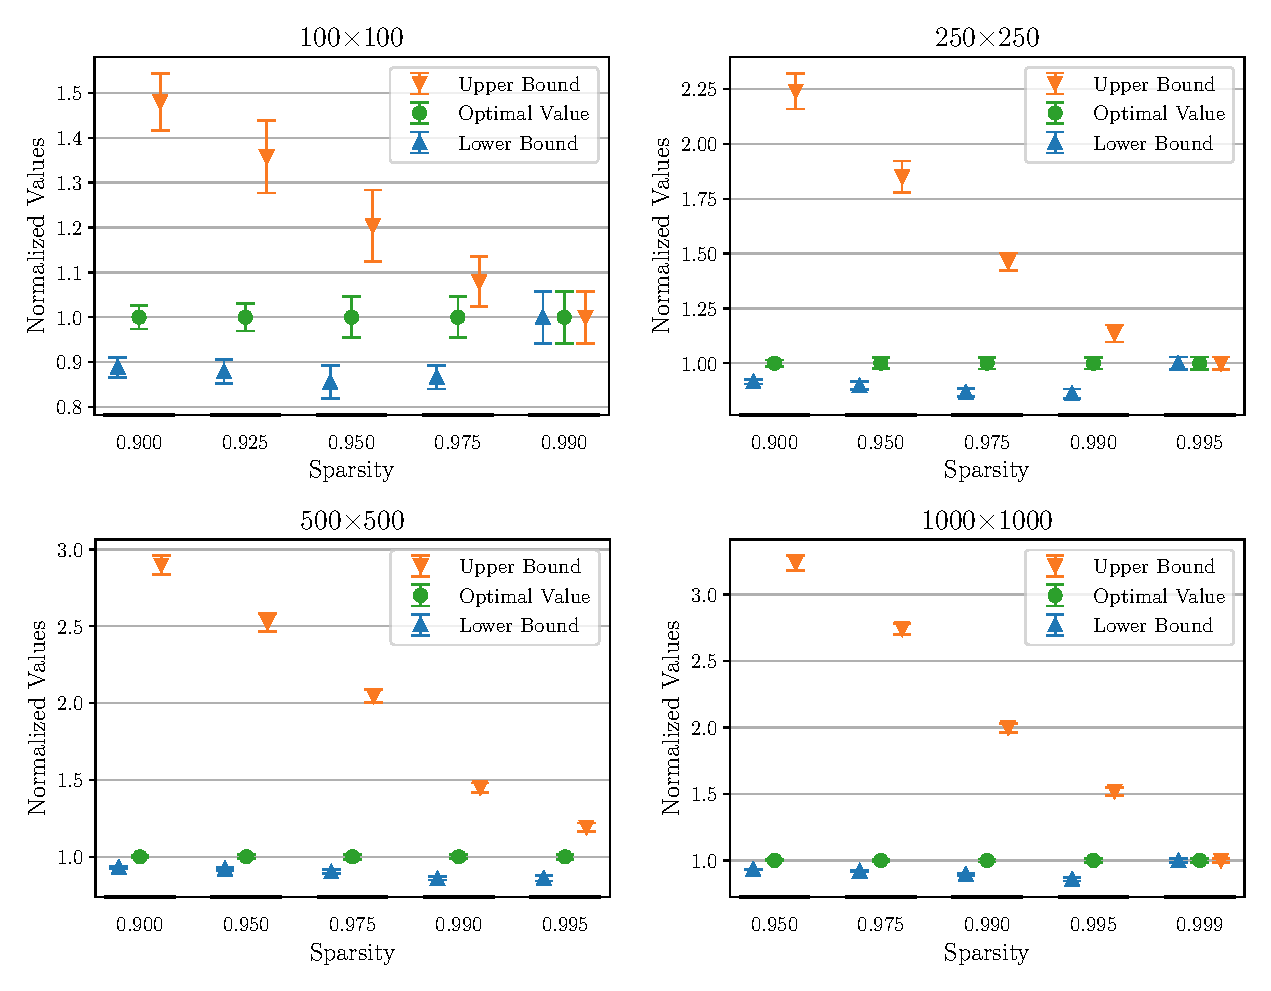
\includegraphics[width=\textwidth]{assets/figures/size.pdf}
    \caption{qualità delle limitazioni prodotte dall'algoritmo di Frank-Wolfe al variare della sparsità e del numero di elementi della
    matrice di riferimento delle istanze.}
    \label{fig:bysize}
\end{figure}

\noindent
Osserviamo che per tutte le istanze che abbiamo scelto, avere un valore di sparsità sufficientemente elevato permette
all'algoritmo di Frank-Wolfe di produrre delle buone limitazioni e, in alcuni casi, anche di chiudere sul valore ottimo
fornito dall'algoritmo del simplesso.
Inoltre, a parità di sparsità, l'aumentare del numero di elementi della matrice di riferimento è indicatore di
un peggioramento nella qualità della limitazione superiore e di un miglioramento nella limitazione inferiore. Il
peggioramento della limitazione superiore è più marcato rispetto al miglioramento della limitazione inferiore, che
rimane invece molto più stabile. Per capire meglio quanto l'aumentare del numero di elementi della matrice di
riferimento influenza le limitazioni prodotte da Frank-Wolfe, abbiamo riportato i valori precisi, ottenuti dallo
svolgimento degli esperimenti, nelle tabelle che seguono.

\begin{table}[!ht]
    \centering
    \begin{tabularx}{300.75005pt}{ccc}
        \toprule
        \text{\alt Dimensione} & \text{\alt Limitazione Inferiore} & \text{\alt Limitazione Superiore} \\
        \midrule
        \( 100\times 100 \) & 0.888 & 1.480 \\
        \( 250\times 250 \) & 0.916 & 2.241 \\
        \( 500\times 500 \) & 0.931 & 2.898 \\
        \bottomrule
    \end{tabularx}
    \caption{valori delle limitazioni prodotte da Frank-Wolfe, normalizzati rispetto al valore ottimo fornito dal
    simplesso, al variare della dimensione delle matrici di riferimento di istanze con sparsità pari a 0.9.}
    \label{table:firstinfo0.9}
\end{table}


\begin{table}[!ht]
    \centering
    \begin{tabularx}{304pt}{ccc}
        \toprule
        \text{\alt Dimensione} & \text{\alt Limitazione Inferiore} & \text{\alt Limitazione Superiore} \\
        \midrule
        \( 100\times 100 \) & 0.855 & 1.204 \\
        \( 250\times 250 \) & 0.899 & 1.850 \\
        \( 500\times 500 \) & 0.920 & 2.525 \\
        \( 1000\times 1000 \) & 0.932 & 3.237 \\
        \bottomrule
    \end{tabularx}
    \caption{valori delle limitazioni prodotte da Frank-Wolfe, normalizzati rispetto al valore ottimo fornito dal
    simplesso, al variare della dimensione delle matrici di riferimento di istanze con sparsità pari a 0.95.}
    \label{table:firstinfo0.95}
\end{table}


\begin{table}[!ht]
    \centering
    \begin{tabularx}{304pt}{ccc}
        \toprule
        \text{\alt Dimensione} & \text{\alt Limitazione Inferiore} & \text{\alt Limitazione Superiore} \\
        \midrule
        \( 100\times 100 \) & 0.867 & 1.080 \\
        \( 250\times 250 \) & 0.867 & 1.462 \\
        \( 500\times 500 \) & 0.903 & 2.047 \\
        \( 1000\times 1000 \) & 0.920 & 2.741 \\
        \bottomrule
    \end{tabularx}
    \caption{valori delle limitazioni prodotte da Frank-Wolfe, normalizzati rispetto al valore ottimo fornito dal
    simplesso, al variare della dimensione delle matrici di riferimento di istanze con sparsità pari a 0.975.}
    \label{table:firstinfo0.975}
\end{table}

\noindent
Il comportamento della limitazione inferiore si inverte quando i valori di sparsità sono molto elevati. In questi casi,
avere matrici più piccole permette di ottenere limitazioni inferiori di qualità migliore e talvolta di chiudere sul
valore ottimo, come evidenziato in precedenza.

\subsection{Forma della matrice di riferimento}
Adesso che abbiamo capito l’influenza della dimensione delle matrici di riferimento sulla qualità delle limitazioni
prodotte dall’algoritmo di Frank-Wolfe, possiamo ripetere gli esperimenti per capire l’impatto della forma della matrice
di riferimento. In particolare, vogliamo capire cosa succede quando il numero delle righe e delle colonne è sbilanciato
da una parte o dall’altra, come accade nella maggior parte delle istanze di problemi di set-covering.

In primo luogo consideriamo matrici di forma differente ma caratterizzate dallo stesso numero di elementi.

\begin{figure}[ht]
    \centering
    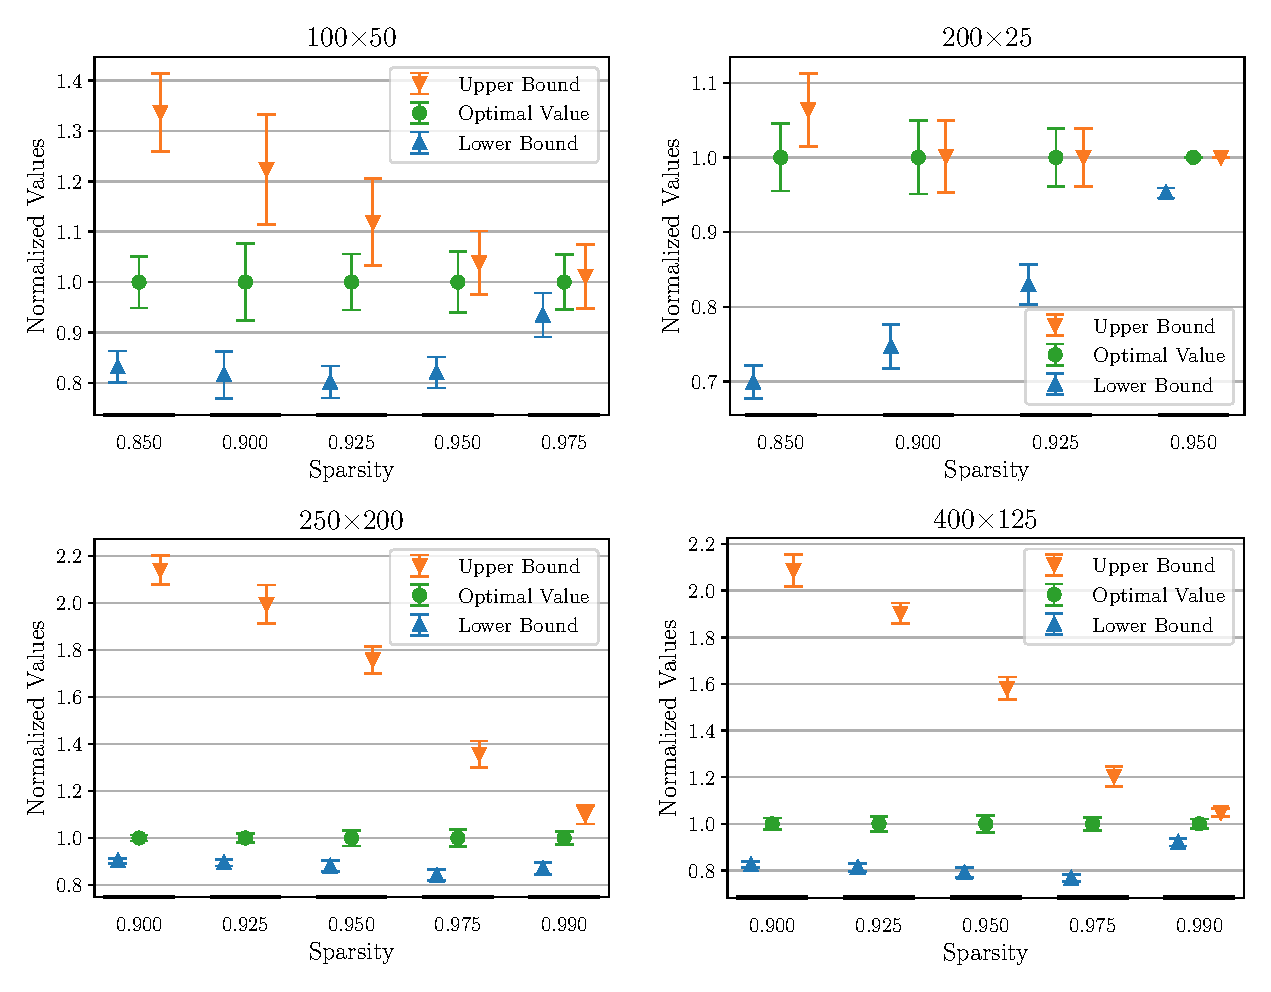
\includegraphics[width=\textwidth]{assets/figures/shape1.pdf}
    \caption{qualità delle limitazioni prodotte dall’algoritmo di Frank-Wolfe al variare della sparsità e della forma
    della matrice di riferimento di istanze piccole e medie.}
    \label{fig:shape1}
\end{figure}

\noindent
I grafici della figura \ref{fig:shape1} mostrano, in ciascuna riga, i risultati ottenuti sperimentalmente dall’esecuzione
dell’algoritmo di Frank-Wolfe su istanze con matrici che hanno lo stesso numero di elementi ma forma differente. Prese
singolarmente, le istanze si comportano come discusso in precedenza: l’aumento della sparsità è indicatore di un
miglioramento della limitazione superiore ma non di quella inferiore, che ha invece un comportamento più irregolare.

Osserviamo che, a parità di sparsità, la forma della matrice influenza i risultati ot- tenuti. In particolare, quando il
numero degli elementi rimane costante si ottengono le limitazioni superiori migliori per le istanze che hanno un numero
di variabili inferiore. Questo risultato è tanto più marcato tanto più sono piccole le istanze che si considerano, come
evidenziato dai risultati della figura \ref{fig:shape2}, relativi a matrici di dimensione maggiore.

\begin{figure}[ht]
    \centering
    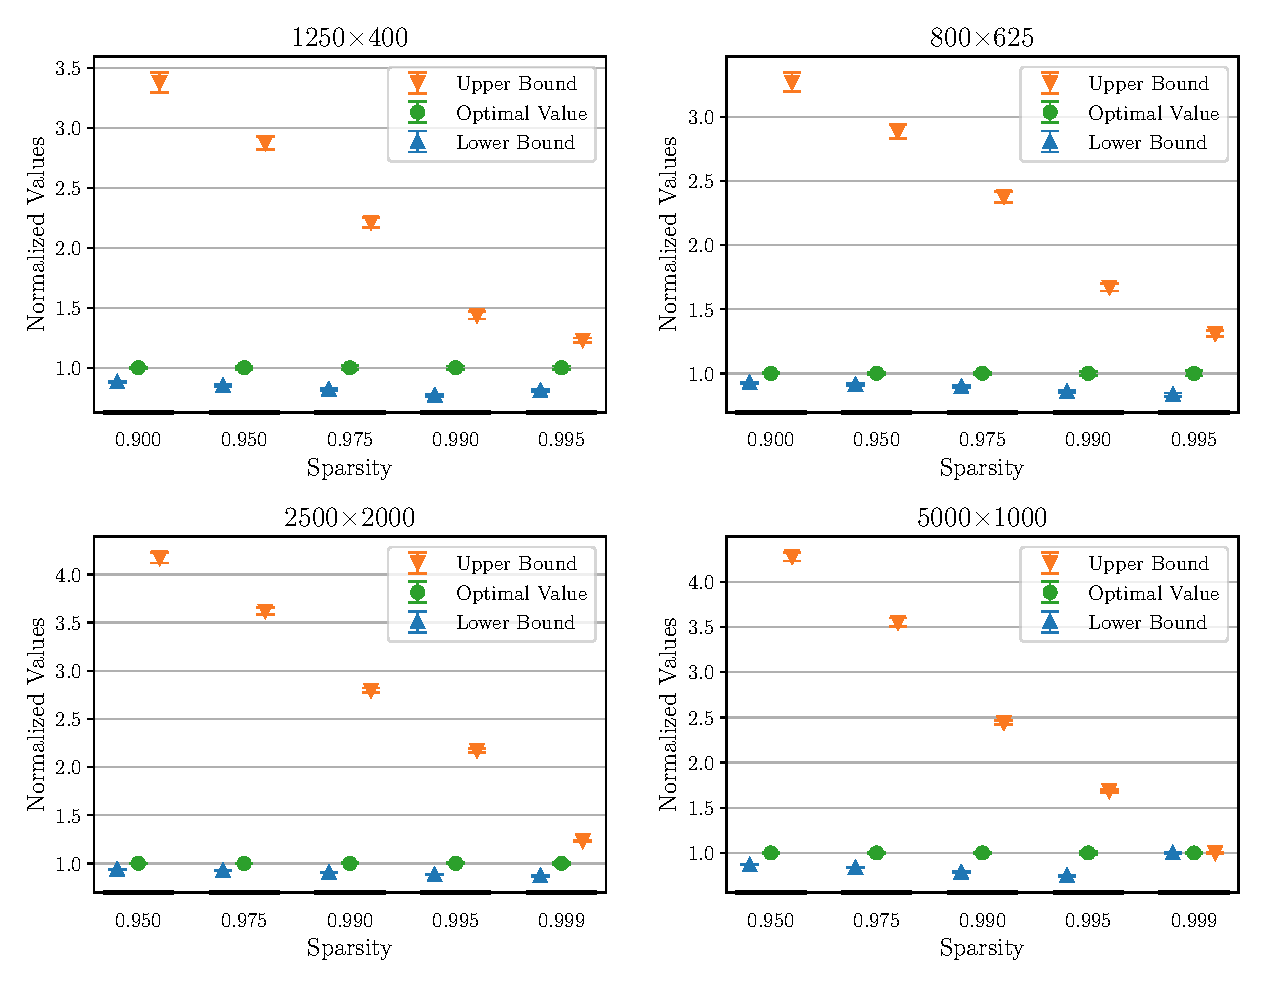
\includegraphics[width=\textwidth]{assets/figures/shape2.pdf}
    \caption{qualità delle limitazioni prodotte dall’algoritmo di Frank-Wolfe al variare della sparsità e della forma
    della matrice di riferimento di istanze grandi.}
    \label{fig:shape2}
\end{figure}

\noindent
Notiamo in questo caso che il comportamento è sempre lo stesso, ma solo per valori di sparsità più elevati. In effetti,
per le matrici 1250 × 400 e 800 × 625 si verifica per sparsità maggiori uguali a 0.950, ma non per valori inferiori, che
individuano un comportamento opposto. Allo stesso modo, per matrici 2500 × 2000 e 5000 × 1000, che sono ancora più
grandi, è necessario avere una sparsità di 0.975 o superiore.

Le limitazioni inferiori sembrano comportarsi in modo opposto. In particolare, si ottengono le limitazioni migliori per
matrici 800 × 625 rispetto a matrici 1250 × 400, a prescindere dalla sparsità. Lo stesso vale per le matrici 2500 ×
2000, che producono limitazioni inferiori migliori rispetto a quanto ottenuto con matrici 5000 × 1000, ma solo quando la
sparsità e inferiore o uguale a 0.995.

In realtà, il comportamento delle limitazioni inferiori sembra dipendere da un altro fattore e non dal numero degli
elementi della matrice. Le limitazioni inferiori non sembra- no dipendere tanto dal numero di elementi o di variabili,
ma piuttosto dal bilanciamento delle matrici. Non è tanto avere un minor numero di variabili che migliora la limitazione
inferiore, ma quanto più avere un numero di variabili che sia bilanciato rispetto al numero dei vincoli. In altre
parole, sperimentalmente si osserva che la qualità delle limitazioni inferiori prodotte dall’algoritmo di Frank-Wolfe è
migliore per le istanze caratterizzate da matrici di riferimento bilanciate, relativamente al numero delle righe e delle
colonne. In effetti, sperimentando ulteriormente si ottengono i risultati della figura \ref{fig:morevars}


\begin{figure}[ht]
    \centering
    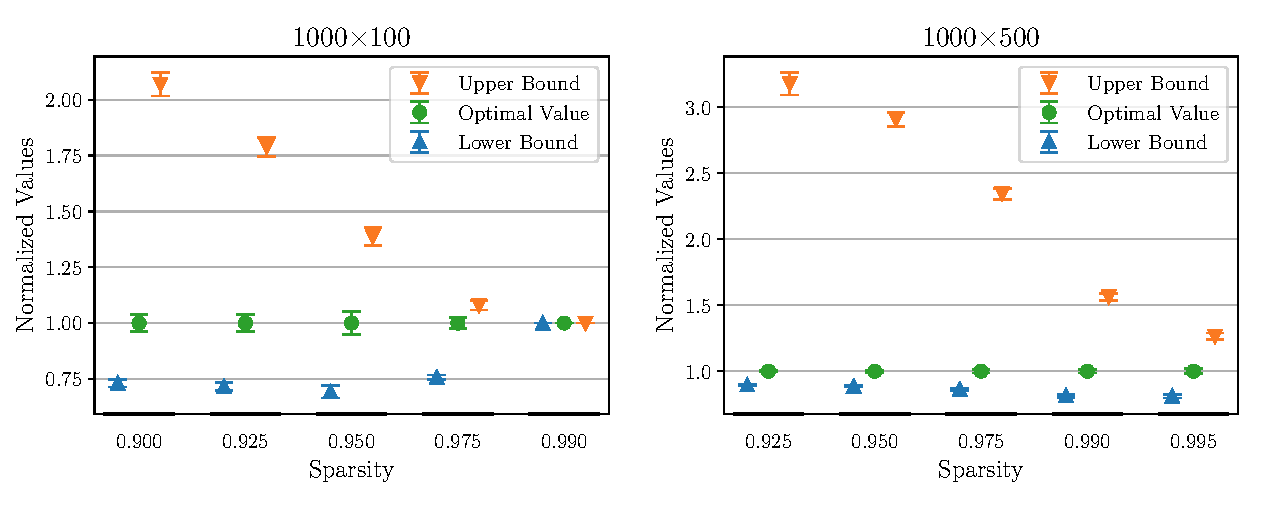
\includegraphics[width=\textwidth]{assets/figures/shape_more_vars.pdf}
    \caption{qualità delle limitazioni prodotte dall'algoritmo di Frank-Wolfe al variare della sparsità e della forma
    della matrice di riferimento.}
    \label{fig:morevars}
\end{figure}

\noindent
Osserviamo che la limitazione superiore si comporta come argomentato in precedenza, migliorando, a parità di sparsità,
per matrici con un numero minore di variabili. La limitazione inferiore invece si comporta diversamente e conferma
quanto ipotizzato, tanto che la qualità è maggiore per le matrici 1000 × 500 quando la sparsità è inferiore o uguale a
0.975. In aggiunta, se confrontiamo i risultati appena ottenuti con quelli della figura 4.1, notiamo che per matrici
1000 × 1000 le limitazioni inferiori sono ancora migliori, a conferma di quanto detto, come evidenziato anche dai dati
riportati per completezza nelle tabelle che seguono.

\begin{table}[!ht]
    \centering
    \begin{tabularx}{300.75005pt}{ccc}
        \toprule
        \text{\alt Dimensione} & \text{\alt Limitazione Inferiore} & \text{\alt Limitazione Superiore} \\
        \midrule
        \( 1000\times 100 \) & 0.715 & 1.788 \\
        \( 1000\times 500 \) & 0.898 & 3.177 \\
        \bottomrule
    \end{tabularx}
    \caption{valori delle limitazioni prodotte da Frank-Wolfe, normalizzati rispetto al valore ottimo fornito dal
    simplesso, al variare della forma delle matrici di riferimento di istanze con sparsità pari a 0.925.}
    \label{table:moreinfo0.925}
\end{table}

\begin{table}[!ht]
    \centering
    \begin{tabularx}{304.39664pt}{ccc}
        \toprule
        \text{\alt Dimensione} & \text{\alt Limitazione Inferiore} & \text{\alt Limitazione Superiore} \\
        \midrule
        \( 1250\times 400 \) & 0.853 & 2.874 \\
        \( 800\times 625 \) & 0.912 & 2.884 \\
        \( 1000\times 100 \) & 0.693 & 1.387 \\
        \( 1000\times 500 \) & 0.887 & 2.907 \\
        \( 5000\times 1000 \) & 0.869 & 4.275 \\
        \( 2500\times 2000 \) & 0.939 & 4.173 \\
        \bottomrule
    \end{tabularx}
    \caption{valori delle limitazioni prodotte da Frank-Wolfe, normalizzati rispetto al valore ottimo fornito dal
    simplesso, al variare della forma delle matrici di riferimento di istanze con sparsità pari a 0.95.}
    \label{table:moreinfo0.95}
\end{table}

\begin{table}[!ht]
    \centering
    \begin{tabularx}{304.39664pt}{ccc}
        \toprule
        \text{\alt Dimensione} & \text{\alt Limitazione Inferiore} & \text{\alt Limitazione Superiore} \\
        \midrule
        \( 1250\times 400 \) & 0.820 & 2.211 \\
        \( 800\times 625 \) & 0.897 & 2.377 \\
        \( 1000\times 100 \) & 0.758 & 1.079 \\
        \( 1000\times 500 \) & 0.862 & 2.344 \\
        \( 5000\times 1000 \) & 0.836 & 3.551 \\
        \( 2500\times 2000 \) & 0.926 & 3.620 \\
        \bottomrule
    \end{tabularx}
    \caption{valori delle limitazioni prodotte da Frank-Wolfe, normalizzati rispetto al valore ottimo fornito dal
    simplesso, al variare della forma delle matrici di riferimento di istanze con sparsità pari a 0.975.}
    \label{table:moreinfo0.975}
\end{table}
Fino a questo momento abbiamo considerato matrici di forme differenti ma in tutti i casi il numero delle colonne era
maggiore uguale al numero delle righe. Questa scelta deriva dal fatto che questa è la condizione più comune per le
istanze del problema del set-covering, in cui il numero dei vincoli è solitamente dominante rispetto al numero delle
variabili. Tuttavia ci sono dei contesti e delle applicazioni in cui potrebbe valere il contrario e quindi abbiamo
effettuato degli esperimenti su matrici in cui il numero delle colonne, ossia il numero di variabili, è maggiore del
numero delle righe, che rappresentano invece i vincoli. I risultati sono riportati nella figura 4.5.

Osserviamo che, a parità di sparsità e numero di vincoli, l'aumentare del numero di variabili è indicatore di un
peggioramento nella qualità della limitazione superiore e di un miglioramento nella qualità della limitazione inferiore.
Se invece consideriamo le matrici che hanno lo stesso numero di variabili accade che, a parità di sparsità, l'aumentare
del numero dei vincoli determina un peggioramento della qualità di entrambe le limitazioni.

Se confrontiamo i risultati ottenuti con matrici caratterizzate dallo stesso numero di elementi ma forme simmetriche,
notiamo che le limitazioni inferiori migliori si ottengono per le matrici in cui il numero delle variabili è dominante
rispetto al numero dei vincoli, come accade ad esempio per le matrici \( 1000\times 500 \) e \( 500\times 1000 \) oppure
\( 2000\times 500 \) e \( 500\times 2000 \). Per le limitazioni superiori la situazione è diversa e l'andamento sembra
dipendere molto dalla sparsità. Ad esempio, per le matrici \( 1000\times 500 \) e
\(
    500\times 1000
\)
la limitazione superiore è migliore quando il numero dei vincoli domina sul numero delle variabili e la sparsità è
inferiore o uguale a 0.975. Per valori di sparsità maggiore il comportamento è opposto e le limitazioni inferiori
migliori sono quelle delle matrici in cui è il numero delle variabili a dominare. Lo stesso comportamento si verifica
per le matrici \( 2000\times 500 \) e  \( 500\times 2000 \), dove la soglia del valore di sparsità è 0.975.

\begin{figure}[ht]
    \centering
    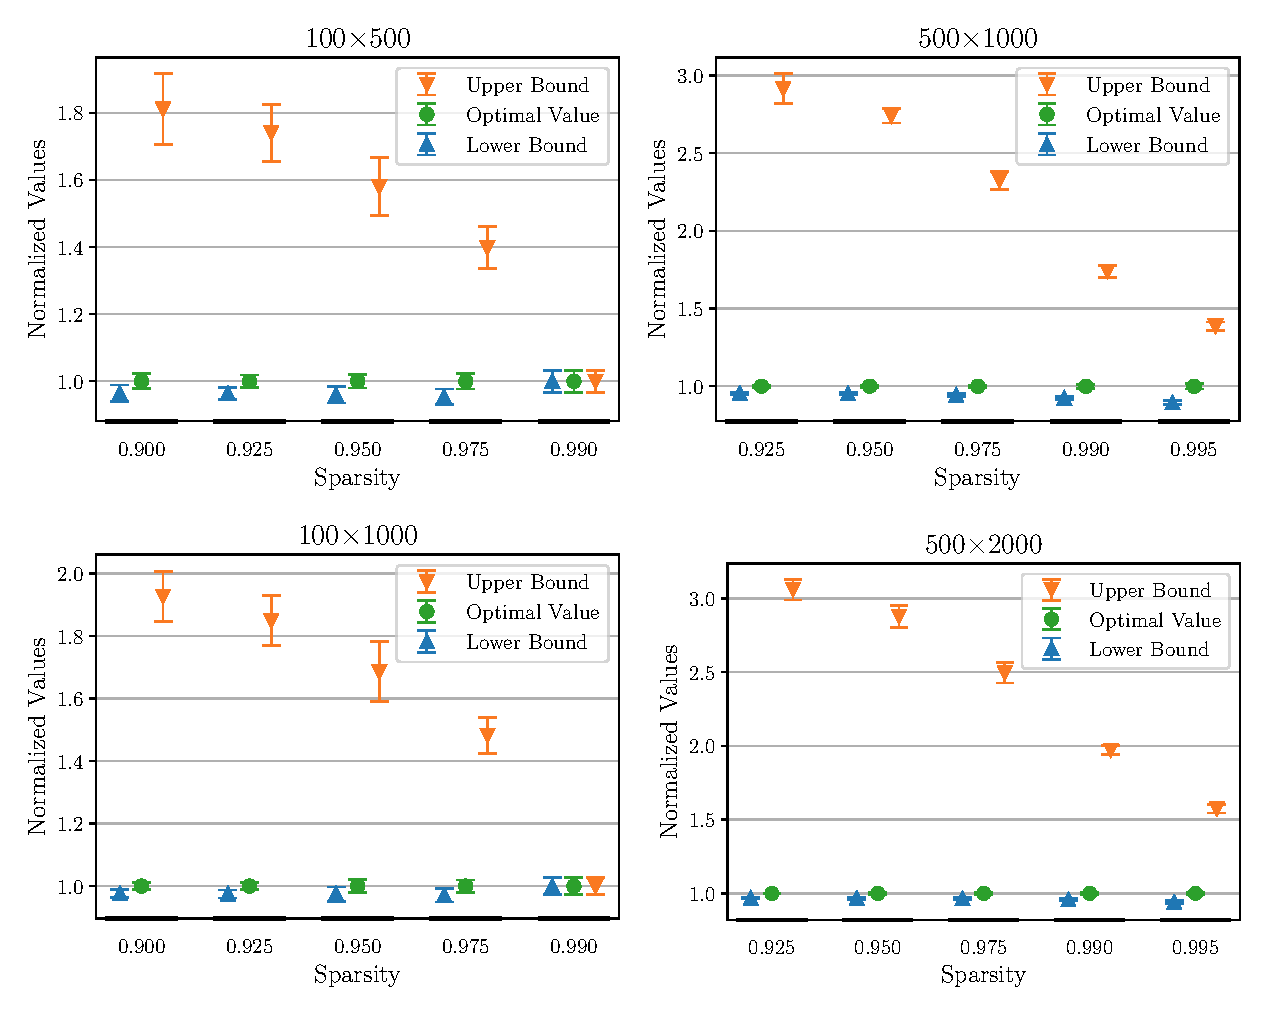
\includegraphics[width=\textwidth]{assets/figures/reverse.pdf}
    \caption{qualità delle limitazioni prodotte dall'algoritmo di Frank-Wolfe al variare della sparsità e della forma
    della matrice di riferimento.}
    \label{fig:reverse}
\end{figure}

\noindent
Le tabelle riportate di seguito evidenziano in modo più chiaro i comportamenti appena osservati.

\begin{table}[!ht]
    \centering
    \begin{tabularx}{300.75005pt}{ccc}
        \toprule
        \text{\alt Dimensione} & \text{\alt Limitazione Inferiore} & \text{\alt Limitazione Superiore} \\
        \midrule
        \( 100\times 500 \) & 0.964 & 1.812 \\
        \( 100\times 1000 \) & 0.976 & 1.927 \\
        \bottomrule
    \end{tabularx}
    \caption{valori delle limitazioni prodotte da Frank-Wolfe, normalizzati rispetto al valore ottimo fornito dal
    simplesso, al variare della forma delle matrici di riferimento di istanze con sparsità pari a 0.9.}
    \label{table:lastinfo0.9}
\end{table}

\begin{table}[!ht]
    \centering
    \begin{tabularx}{300.75005pt}{ccc}
        \toprule
        \text{\alt Dimensione} & \text{\alt Limitazione Inferiore} & \text{\alt Limitazione Superiore} \\
        \midrule
        \( 100\times 500 \) & 0.964 & 1.741 \\
        \( 100\times 1000 \) & 0.975 & 1.850 \\
        \( 500\times 1000 \) & 0.954 & 2.915 \\
        \( 500\times 2000\) & 0.969 & 3.059 \\
        \bottomrule
    \end{tabularx}
    \caption{valori delle limitazioni prodotte da Frank-Wolfe, normalizzati rispetto al valore ottimo fornito dal
    simplesso, al variare della forma delle matrici di riferimento di istanze con sparsità pari a 0.925.}
    \label{table:lastinfo0.925}
\end{table}

\begin{table}[!ht]
    \centering
    \begin{tabularx}{300.75005pt}{ccc}
        \toprule
        \text{\alt Dimensione} & \text{\alt Limitazione Inferiore} & \text{\alt Limitazione Superiore} \\
        \midrule
        \( 100\times 500 \) & 0.960 & 1.580 \\
        \( 100\times 1000 \) & 0.975 & 1.687 \\
        \( 500\times 1000 \) & 0.952 & 2.741 \\
        \( 500\times 2000\) & 0.967 & 2.877 \\
        \bottomrule
    \end{tabularx}
    \caption{valori delle limitazioni prodotte da Frank-Wolfe, normalizzati rispetto al valore ottimo fornito dal
    simplesso, al variare della forma delle matrici di riferimento di istanze con sparsità pari a 0.95.}
    \label{table:lastinfo0.95}
\end{table}

\begin{table}[!ht]
    \centering
    \begin{tabularx}{300.75005pt}{ccc}
        \toprule
        \text{\alt Dimensione} & \text{\alt Limitazione Inferiore} & \text{\alt Limitazione Superiore} \\
        \midrule
        \( 100\times 500 \) & 0.953 & 1.398 \\
        \( 100\times 1000 \) & 0.971 & 1.482 \\
        \( 500\times 1000 \) & 0.944 & 2.324 \\
        \( 500\times 2000\) & 0.964 & 2.496 \\
        \bottomrule
    \end{tabularx}
    \caption{valori delle limitazioni prodotte da Frank-Wolfe, normalizzati rispetto al valore ottimo fornito dal
    simplesso, al variare della forma delle matrici di riferimento di istanze con sparsità pari a 0.975.}
    \label{table:lastinfo0.975}
\end{table}

\begin{table}[!ht]
    \centering
    \begin{tabularx}{300.75005pt}{ccc}
        \toprule
        \text{\alt Dimensione} & \text{\alt Limitazione Inferiore} & \text{\alt Limitazione Superiore} \\
        \midrule
        \( 500\times 1000 \) & 0.925 & 1.739 \\
        \( 500\times 2000\) & 0.958 & 1.972 \\
        \bottomrule
    \end{tabularx}
    \caption{valori delle limitazioni prodotte da Frank-Wolfe, normalizzati rispetto al valore ottimo fornito dal
    simplesso, al variare della forma delle matrici di riferimento di istanze con sparsità pari a 0.99.}
    \label{table:lastinfo0.99}
\end{table}

\begin{table}[!ht]
    \centering
    \begin{tabularx}{300.75005pt}{ccc}
        \toprule
        \text{\alt Dimensione} & \text{\alt Limitazione Inferiore} & \text{\alt Limitazione Superiore} \\
        \midrule
        \( 500\times 1000 \) & 0.895 & 1.387 \\
        \( 500\times 2000\) & 0.940 & 1.575 \\
        \bottomrule
    \end{tabularx}
    \caption{valori delle limitazioni prodotte da Frank-Wolfe, normalizzati rispetto al valore ottimo fornito dal
    simplesso, al variare della forma delle matrici di riferimento di istanze con sparsità pari a 0.995.}
    \label{table:lastinfo0.995}
\end{table}

\section{Tempi di esecuzione}
Gli esperimenti che abbiamo condotto fino a questo punto ci hanno permesso di capire come si comporta l'algoritmo di
Frank-Wolfe al variare dei parametri che identificano le istanze che abbiamo considerato, come ad esempio la sparsità,
il numero di elementi e la forma della matrice di riferimento. In particolare, abbiamo cercato di stabilire la qualità
delle limitazioni prodotte da Frank-Wolfe confrontandole con il valore ottimo ottenuto attraverso l'algoritmo del
simplesso. Analizzando i risultati che abbiamo ottenuto, siamo riusciti a concludere che la limitazione inferiore e
quella superiore si comportano diversamente. In particolare, la prima è molto più stabile della seconda, al variare dei
parametri che abbiamo considerato. In generale, abbiamo ottenuto delle limitazioni ragionevoli che richiedono ora di
confrontare il tempo impiegato per ottenerle con il tempo necessario a trovare la soluzione ottima con l'algoritmo del
simplesso. L'obiettivo è quello di capire se l'algoritmo di Frank-Wolfe è in grado di produrre limitazioni di buona
qualità in un tempo molto ridotto.

In questa sezione analizzeremo i tempi di esecuzione dei due algoritmi, al variare dei parametri che abbiamo
citato in precedenza. Per l'algoritmo del simplesso considereremo il tempo impiegato a trovare il valore ottimo, mentre
per l'algoritmo di Frank-Wolfe considereremo il tempo impiegato a compiere un numero di iterazioni fissato. L'idea è
quella di eseguire l'algoritmo di Frank-Wolfe molteplici volte per capire come il numero di iterazioni influenza le
limitazioni prodotte. L'obiettivo è quello di trovare un compromesso tra la qualità delle limitazioni prodotte e il
tempo impiegato per ottenerle, in relazione al tempo necessario per determinare il valore ottimo attraverso l'algoritmo
del simplesso.

\section{Dimensione della matrice di riferimento}
Iniziamo analizzando i risultati ottenuti dagli esperimenti svolti su istanze di dimensioni
differenti, in quanto a numero di elementi della matrice di riferimento, che sono riportati nei grafici della figura
\ref{fig:timesize}.

\begin{figure}[!ht]
    \centering
    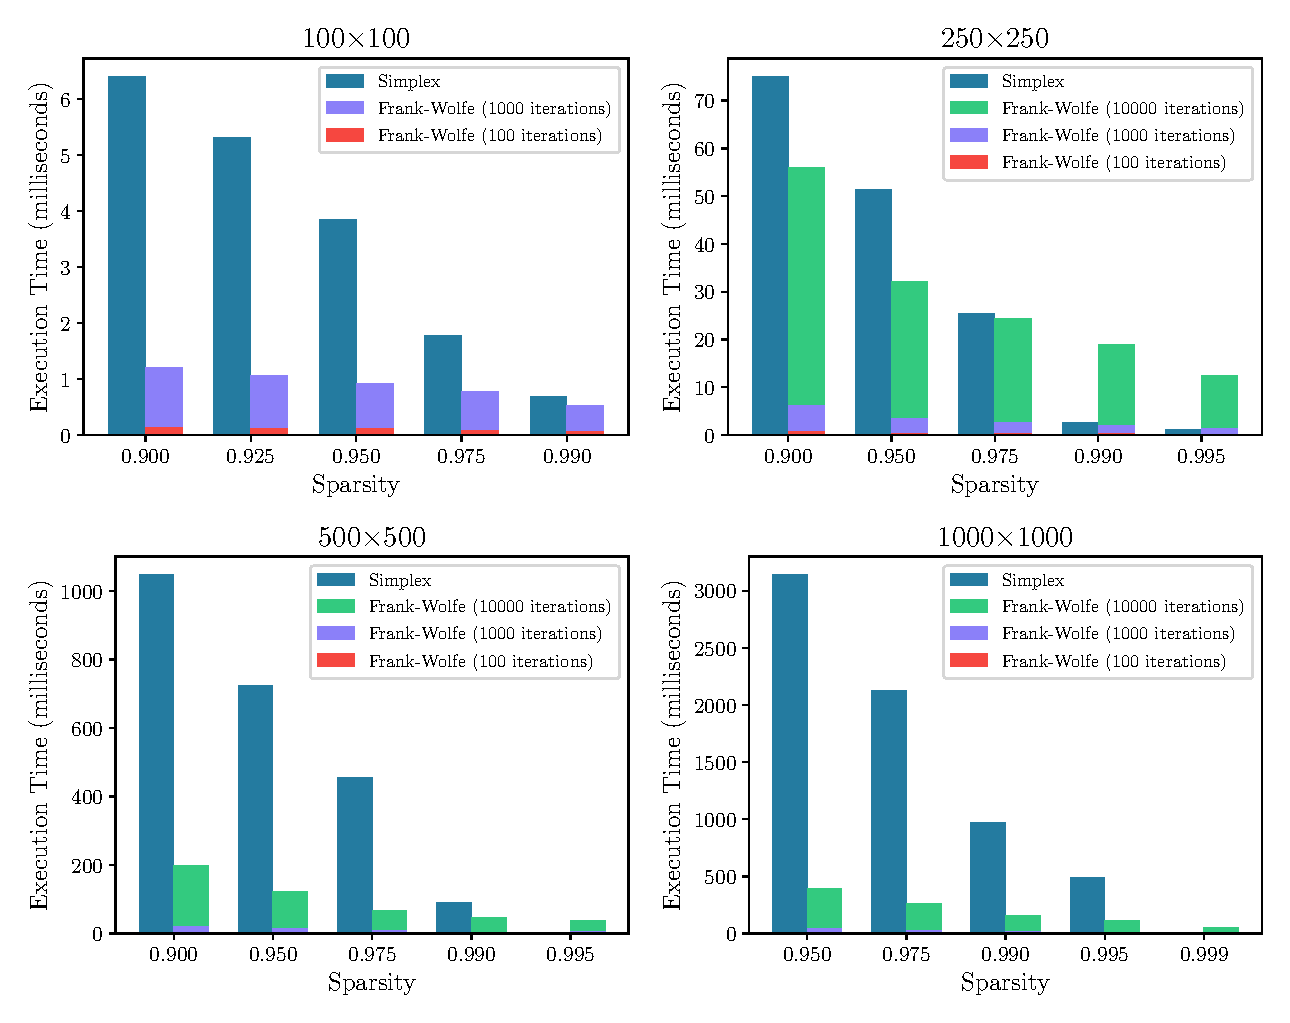
\includegraphics[width=\textwidth]{assets/figures/timesize.pdf}
    \caption{tempi di esecuzione dell'algoritmo del simplesso e dell'algoritmo di Frank-Wolfe, al variare della sparsità
    e della dimensione della matrice di riferimento.}
    \label{fig:timesize}
\end{figure}

In primo luogo notiamo che la sparsità della matrice ha un'influenza significativa sul tempo di esecuzione
dell'algoritmo del simplesso.  In particolare,
l'aumento della sparsità è indicatore di una diminuzione del tempo di esecuzione.
Per l'algoritmo di Frank-Wolfe l'effetto è il medesimo, ma è meno marcato.
Naturalmente
questo risultato non è una sorpresa, poiché più è sparsa una matrice e minore sarà il numero di operazioni da eseguire.

Per matrici di riferimento abbastanza piccole, i tempi di esecuzione degli algoritmi sono molto bassi e quindi
c'è poco spazio per le variazioni. Tuttavia, quando la matrice di riferimento è sufficientemente grande, notiamo proprio
una soglia di sparsità oltre la quale l'algoritmo del simplesso è incredibilmente più veloce. L'andamento dei tempi di
esecuzione dell'algoritmo Frank-Wolfe è invece molto più stabile.

Se confrontiamo i tempi di esecuzione dei due algoritmi possiamo osservare che per matrici piccole l'algoritmo di
Frank-Wolfe si comporta molto bene, con tempi di esecuzione ridotti rispetto a quelli dell'algoritmo del
simplesso, soprattutto per i valori di sparsità più bassi. Per i valori di sparsità più elevati, l'algoritmo di
Frank-Wolfe rimane competitivo solo quando il numero di iterazioni è ridotto, come accade ad esempio per le matrici \(
250\times 250 \). Per matrici di dimensione maggiore e valori di sparsità contenuti, il tempo di esecuzione del simplesso aumenta notevolmente, mentre
quello dell'algoritmo di Frank-Wolfe aumenta in modo meno significativo. Al contrario, valori molto elevati di
sparsità velocizzano di molto l'esecuzione del simplesso, i cui tempi si abbassano di molto rispetto a quelli
dell'algoritmo di Frank-Wolfe.

Osserviamo poi che il numero delle iterazioni effettuate dall'algoritmo di Frank-Wolfe ha un influenza significativa sul
tempo di esecuzione. Per questo motivo, è importante capire quanto migliora la qualità delle limitazioni prodotte,
all'aumentare del numero di iterazioni.
